
В области определения позы животных проделано сильно меньше работы, чем в этой же области для людей. Причины очевидны:
\begin{itemize}
    \item Широкий потенциал применения
    \item Возможность использовать актёров
    \item Большое количество фотографий
\end{itemize}
\subsection{На людях} \label{subsect1_3_1}
Сейчас классификацию позы людей осуществляют с помощью так называемого Pose Estimation Tree. Целью зрения становится будто восстановить человеческий скелет по изображению. Для этого определяются важные подвижные узлы - joints. Обычно ими являются локти, колени и другие суставы. У человека всего порядка 200 таких узлов. При этом при решении большинства задач компьютерного зрения используется около 20.
\begin{figure}[ht] 
  \center
  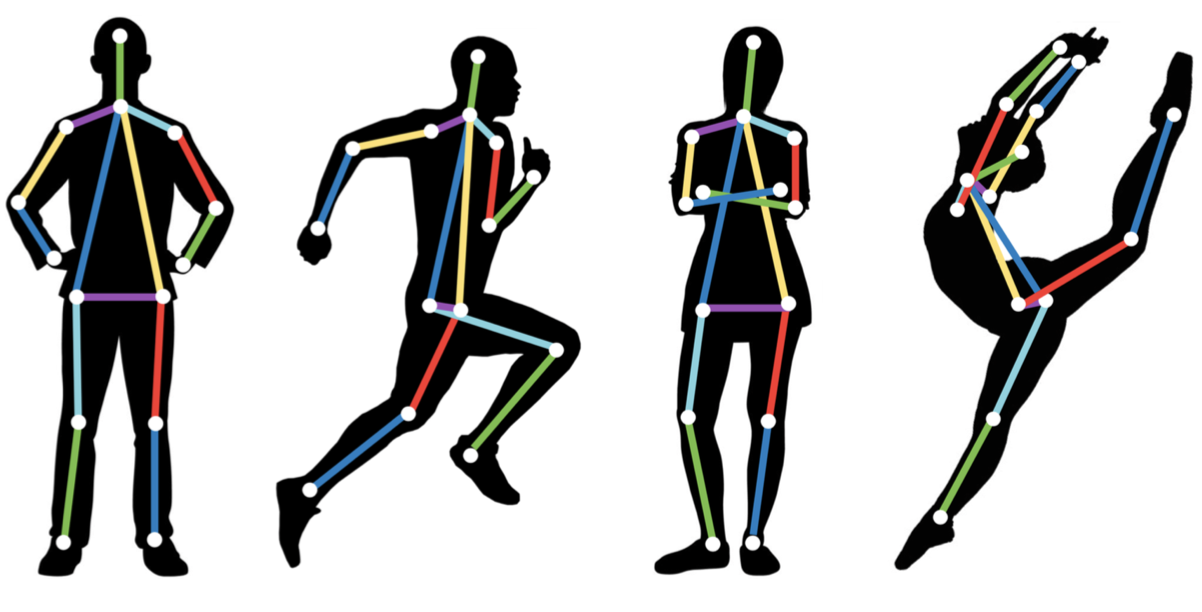
\includegraphics [width=\textwidth/2] {pose}
  \caption{Pose Estimation Tree} 
  \label{img:poseest}  
\end{figure}

Классические пакетные решения для такой задачи - Tensorflow Pose Kit и OpenPose. Всё что требуется для этих пакетов - набор размеченных данных для обучения. OpenPose может работать с множественными объектами и окклюзиями, но относительно медленный. Tensorflow Pose Kit создан с уклоном в перенос модели на портативные устройства.

В статье выпускников Стенфорда 2015 года советуется использовать классификацию деятельности строго отдельно от задачи получения дерева конечностей человека, а не одно на результатах другого.\cite{Bearman2015HumanPE} Основная причина в том, что дерево конечностей крайне нестабильно, его точность далека от идеальной и от окклюзий конечностей самим человеком практически нельзя избавиться. В подтверждение этому, на 20 классах активности, они добились точности в 80\% без использования pose estimation, что считается хорошо для такого большого количества классов.

\subsection{На животных} \label{subsect1_3_2}
В 2018 году вышла публикация \cite{deeplabcut}, в которой авторы предложили новаторский способ автоматически следить за указанными частями тела у животных. Алгоритму не требуется больших датасетов с данными, нужно всего около 200 кадров (от 8 секунд видео) чтобы предсказать остальной видеопоток. 
\begin{figure}[ht] 
  \center
  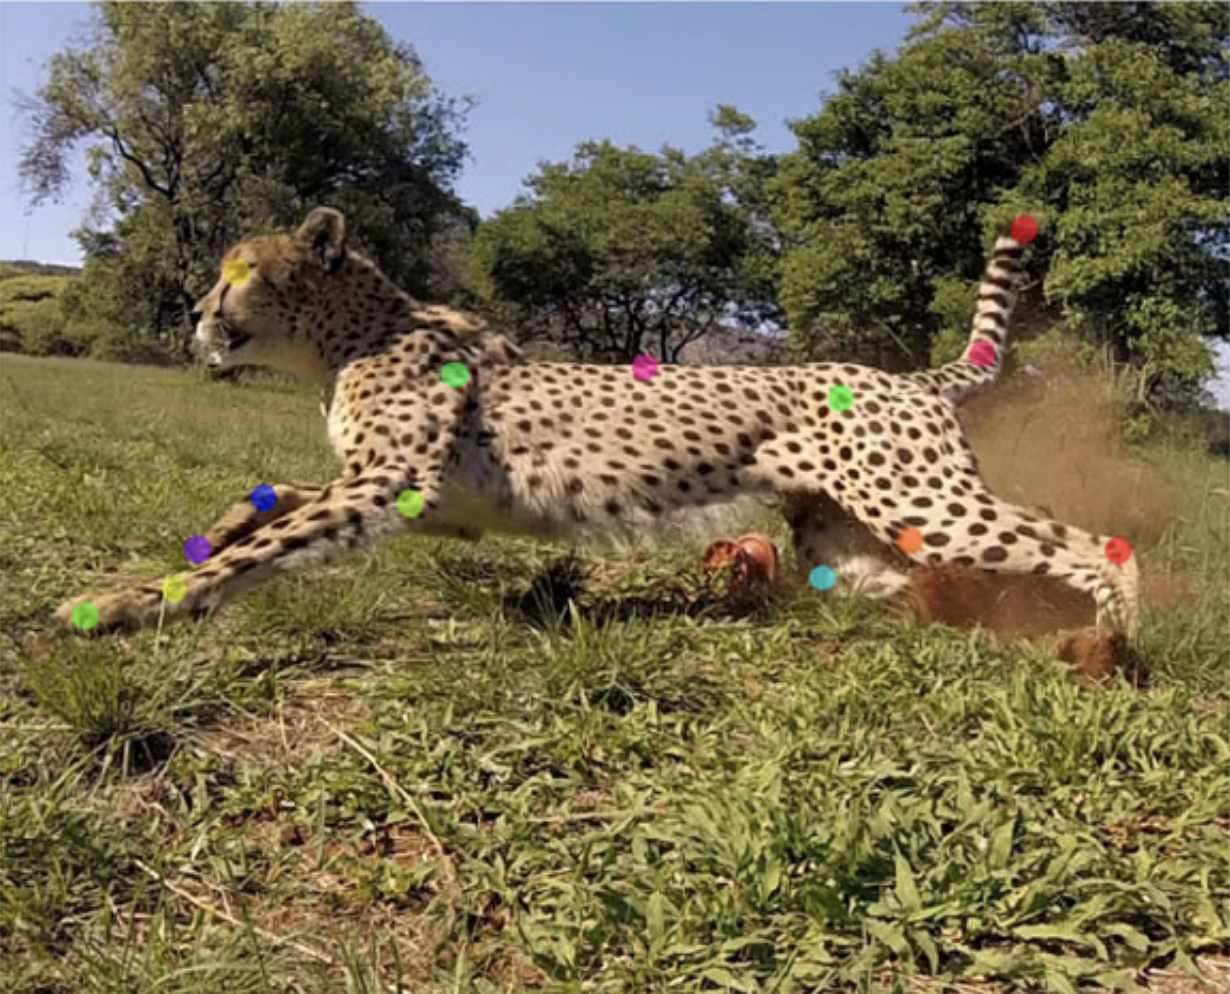
\includegraphics [width=\textwidth/2] {deeplabcut}
  \caption{Предсказанный кадр DeepLabCut} 
  \label{img:deeplabcut}  
\end{figure}
Ограничениями данного метода являются необходимость в разметке этих первых 200 кадров, на это уходит обычно около 20 минут, а также принципиальная возможность работать только с видеопотоком. 
В итоге это достаточно хороший метод для того чтобы разметить большие видеопотоки. Алгоритм обеспечивает достаточную точность и на длинных видеозаписях позволяет сильно сократить время на разметку данных для Pose Tree Estimation. Применение данного способа не ограничивается только на животных: любой видеопоток, на котором можно отслеживать объекты будет работать.
